\section{Специфика систем накопления энергии в разработке систем управления}


Как было описано в разделе \ref{sec:references}, в целевой физической системе все отклонения от предсказанных мощностей потребления и генерации компенсируются одним специально выделенным устройством --- первичным накопителем.
Назовём такую систему \textit{монобалансирующей}.
В монобаласирующей системе существует вероятность вероятность нежелательных перетоков энергии из первичного накопителя во вторичный и обратно, то есть циклы мощности внутри системы накопления энергии, как схематически изображено на Рис \ref{fig:power_flow_graph}.
Рассмотрим ситуацию, когда разность между мощностью нагрузки и мощностью ветрогенерации $P_{req}$  колеблется около нуля с периодом порядка периода выбора уставок.
Тогда, при неудачном выборе уставок мощности для вторичного накопителя (например, при прогнозе ветра равном среднему за предыдущий период) 
может получиться такой режим (см Рис \ref{fig:bad_batteries}),
что вторичный накопитель то заряжается от первичного в то время, как $P_{req} > 0$; то разряжается в первичный при $P_{req} < 0$ .


\begin{figure}[]
\begin{tikzpicture}[shorten >=1pt,node distance=2cm,on grid,auto]
  \tikzstyle{every state}=[fill={rgb:black,1;white,10}]

  \node[state, minimum size=2.2cm]  (w) at (0, 0)     {ветер};
  \node[state, minimum size=2.2cm]  (l) at (4, 0)     {нагрузка};
  \node[state, minimum size=2.2cm]  (s) at (2, -3)  {накопители};

  \path[->]
  (w) edge                node {}  (l)
  (w) edge                node {}  (s)
  (s) edge                node {$P_L$}  (l)
  (s) edge  [loop below]  node {$P_{ps}, P_{sp}$}  ();
\end{tikzpicture}
\centering
\caption{Диаграмма перетоков мощности}
\label{fig:power_flow_graph}
\end{figure}

\begin{figure}[]
\includegraphics[scale=0.65]{/bad_batteries.png}
\centering
\caption{Плохой случай для системы с одним балансирующим устройством. Мощность нагрузки постоянна и равна 50кВт}
\label{fig:bad_batteries}
\end{figure}

Это приводит к лишнему износу накопителей и потерям энергии из-за $\eta < 1$.
Заметим, что в данном конкретном случае есть два принципиально различных ``хороших'' режима: 
\begin{enumerate}
    \item  Уставка вторичного накопителя $\equiv  0$.
    Все колебания сглаживаются первичным накопителем. 
    \item Вторичный накопитель идеально подстраивается под профиль ветра, первичный реагирует только на отклонения $P_{req}$ от своего среднего за период.
\end{enumerate}

У второго варианта два существенных недостатка: 
необходимость знать будущее и сохранение (неустранимой для монобалансирующей системы) проблемы с перетоками мощности в случае значительной дисперсии $P_{req}$ в периодах между обновлением уставок.
Недостаток первого варианта в том, что логически первичный накопитель предназначен только для компенсации колебаний внутри периода между выбором уставок.
В данном частном случае это исправляется увеличением этого периода вдвое.

Монобалансирующая система, использующая прогноз по предыдущему периоду, хороша тем, что с ней практически не нужно заботиться о поддержании заряда первичного накопителя в допустимом диапазоне:


% Поэтому достаточно, чтобы ширина рабочего диапазона опорно-балансирующей батареи $E_{core}(SoE_{max} - SoC_{min})$ была больше $\left(P_{req~max} - P_{req~min}\right)\Delta t$, тогда начало работы с состояния 
% $E_{core}(SoE(0) - SoC_{min}) = \left(P_{req}(i) - P_{req~max}\right)\Delta t $ гарантирует, что SoC будет находиться допустимом диапазоне при $\eta = 1$.
% При $\eta < 1$ нужно будет периодически подзаряжать опорно-балансирующую батарею для компенсации потерь.

Далее будем считать, что система работает без дизель-генератора, и что разность между ветрогенерацией и нагрузкой $P_{req}$ всегда можно удовлетворить за счёт вторичного накопителя, или  $P_{req}$ скорректирована таким образом, чтобы под них подходить (это нужно, чтобы не думать сейчас о случаях, когда, например, ветра слишком много и вторичный накопитель уже заряжен).  
Для простоты учёта баланса мощности будем также считать, что КПД накопителей равен 1 (хотя потери при перетоках между накопителями~--- как раз то, что заставляет нас рассматривать эту проблему).

Главный вопрос об эффективности монобалансирующих системах, который нас интересует: для каких $\alpha$ существует управление (уставка вторичному накопителю с отрицательным знаком, то есть положительная при разряде) $u(i) = f(P_{req}(0), \ldots, P_{req}(i-1))$, $E_{p}(SoE(i) - SoC(i-1)) = \left( u(i) - P_{req}(i)\right)\Delta t$ удовлетворяющее следующим условиям (*):
\begin{enumerate}
    \item $\forall i ~ SoE(i) \in [SoC_{min}, SoC_{max}] \eqdef [0, 1]$ (для удобства производим перемасштабирование, чтобы считать ширину допустимого диапазона равной ёмкости первичного накопителя) .
    \item Ограничение на максимально допустимую долю энергии, перешедшую из одной батареи в другую: $E_{ps} + E_{sp} < \alpha E_{L}  ~\forall \Vec{P}_{req}$, здесь $E_{ps}, E_{sp}$ --- энергия поступившая из первичного накопителя во вторичный и обратно, соответственно; 
  % мб $E_{L} + E_f$ ??
    $E_{L}$ ---  энергия, отданная нагрузке системой аккумуляторов.
    Это ограничение соответствует ограничению на потери энергии в ходе циклических перетоков мощности между накопителями.
\end{enumerate}

Здесь $p$ в индексах соответствует первичному накопителю (primary), $s$~--- вторичному (secondary).

% Рассмотрим режим работы, в котором дизель-генератор выключен и нагрузка обеспечивается батареей гибкости и ветрогенерацией.
% Идеализируем эту систему, предполагая, что начальная энергия батареи гибкости = 0, диапазон энергий = $(-\infty, \infty)$ (бесконечная ёмкость, бесконечный запас энергии в начальный момент).
Считая, как обычно, что мощность батареи положительна при заряде, в использованных выше обозначениях для данного случая получаем $u = -P_{s}$.
Тогда 

\begin{equation}
\label{f:Efc}
\frac{dE_{sp}}{dt} = 
\begin{cases}
u,& P_{req} \leq 0, u \geq 0,\\
ramp(u - P_{req}),& P_{req} \geq 0, u \geq 0,\\
0,& u \leq 0.
\end{cases}
\end{equation}

И, аналогично

\begin{equation}
\label{f:Ecf}
\frac{dE_{ps}}{dt} = 
\begin{cases}
-u,& P_{req} \geq 0, u \leq 0,\\
ramp(P_{req} - u),& P_{req} \leq0, u \leq 0,\\
0,& u \geq 0.
\end{cases}
\end{equation}

Здесь $ramp$~---функция, равная нулю, если агрумент отрицателен, и равная своему аргументу в противном случае. 
% Легко заметить, что при $P_{req}(i) = -u$

% 3 дня работы деградированного интеллекта студента 6 курса
Понятно, что при $P_{req} \equiv 0$, если были какие-то потоки энергии, то в условии 2 $\alpha = 1$. 
Но в таком случае при $u \equiv 0 $ будут нулевые перетоки энергии. 
Поэтому учитывать стоит только случаи, когда левая и правая части условия растут с течением времени.
Легко заметить, что справедливо следующее
\begin{Statement}
Пусть в начальный момент времени энергия опорной батареи находилась в середине допустимого интервала, система монобалансирующая с \textit{фиксированным} шагом времени.
Пусть $\forall i ~P_{req}(i) \in [P_{req~min}, P_{req~max}] \eqdef [-A, A]$. 
Тогда $\forall u$, удовлетворяющего (*), существует $P_{req}$ такое, что сумма $E_{ps} + E_{sp}$ неограниченно растёт с течением времени, и в условии 2 выполнено $\alpha > 0.5 = \alpha_0$.
\end{Statement}


\begin{proof}
Возьмём произвольное управление $u$, удовлетворяющее (*).
Построим для него такой профиль разности между нагрузкой и ветрогенерацией $P_{req}$, чтобы было выполнено \begin{equation}
\label{f:a_0}
    E_{ps} + E_{sp} \geq \alpha_0 E_{L}.
\end{equation}

Пусть $u(i) = f(P_{req}(0), \ldots, P_{req}(i-1))$. 
Положим $$
P_{req}(i) = \begin{cases}
A\cdot \sign(\frac{1}{2} - SoE_{p}), &|u_i| \leq \frac{A}{2}~ (i \in \I),\\
0, &|u_i| \geq \frac{A}{2}~ (i \in \K).
\end{cases}
$$
Обозначим $\Delta E(i)$ изменение энергии первичного накопителя на i-ом шаге.
Так как при $i \in \I$ $P_{req}$ старается увести SoE первичного накопителя за границы допустимого диапазона, то понятно, что
$$\sum_{i \in \K}{|\Delta E(i)|} \geq \sum_{i \in \I}{|\Delta E(i)|} -\frac{E_{p}}{2} ,$$
здесь $E_p$~--- ширина допустимого диапазона.
Это особенно очевидно, если воспользоваться симметрией допустимого диапазона относительно 0.5 (считать, что при переходе через 0.5 сверху вниз траектория энергии отражается), тогда на шагах из $\I$ SoE движется всегда вверх, а на шагах из $\K$ может двигаться в любом направлении.

Воспользовавшись этим и \ref{f:Efc}-\ref{f:Ecf}, получаем

$$
E_{fc} + E_{cf} %\geq \Delta t \sum_{i \in \K}{|u_i|} 
\geq \sum_{i \in \K}{|\Delta E(i)|} \geq 
\sum_{i \in \I}{|\Delta E(i)|} -  \frac{E_{p}}{2} \geq
\frac{1}{2} E_{L} - E_{p}.
$$
Первое неравенство следует из того, что на шаге с номерами $i \in \K$ нагрузка равна ветрогенерации, поэтому на изменение уровня энергии в первичном накопителе накопителе на этом шаге равно перетоку энергии между накопителями.
В последнем неравенстве используется, что обмен мощностью с системой накопления происходит только на шагах из $\I$, и энергия, переданная от системы накопления нагрузке составляет не менее половины энергии, просуммированной по всем обменам с системой накопления за вычетом, быть может, ширины допустимого интервала.


% Пусть прошло $k$ периодов.
% Обозначим $n \defeq |\mathcal{I}|,~ \mathcal{I} \defeq \{i : |u(i)| \leq A/2, i\leq k\}$, 
% $m \defeq |\mathcal{K}|,~ \mathcal{K} \defeq \{i : |u(i)| \geq A/2, i \leq k\}$.

% Докажем, что $n \leq 4m$.
% При $i \in \mathcal{I}$ энергия опорной батареи изменяется (по модулю) на величину $\Delta E \geq \frac{A}{2} \Delta t$ в сторону ближайшей границы допустимого интервала.
% При $i \in \mathcal{K}$ энергия меняется на величину $ \Delta E \leq 2A \Delta t$ в произвольную сторону.
% Отсюда очевидно, что при $n > 4m$ (с учётом начального условия) энергия батареи выходит за границы допустимого интервала, поэтому приходим к противоречию.

% Так как $E_{L} + E_f \leq \sum_i^k{|u(i)|}$ \textit{(мб можно улучшить оценку?)} и  при каждом $i \in \mathcal{K}$ выполнено $ E_{cf}(i) + E_{fc}(i) = |u(i)| \geq \frac{A}{2}$, то 
Из этого следует справедливость \ref{f:a_0} для $\alpha_0 = \frac{1}{2}$.
\end{proof}

Полученный результат говорит о том, что не существует системы управления монобалансирующей системой со многоуровневой системой накопления энергии, для которой перетоки мощности между накопителями были бы пренебрежимо малы при любых внешних условиях: в худшем случае не менее 50\% от энергии, поступающей в систему накопления испытывает двойные потери за счёт обмена энергией между накопителями.
Выводы из этого следующие:

\begin{enumerate}
    \item В качестве варианта по-умолчанию стоит рассматривать системы, где функции первичного и вторичного накопителя объединены в одном литий-ионном аккумуляторе.
    
    \item При создании систем с гибридной системой накопления энергии необходим анализ ожидаемых временных рядов разности ветрогенерации и нагрузки $P_{req}$, чтобы выбором параметров алгоритма управления по возможности минимизировать перетоки между накопителями (выбрать период между выбором уставок таким, чтобы циклы выбора уставок не накладывались на циклы $P_{req}$, убедиться в возможности минимизации перетоков). 
    
    \item При проектировании локальных системы управления устройствами силовой электроники следует закладывать возможность динамического изменения коэффициентов статизма, чтобы все накопители могли откликаться на колебания $P_{req}$ до вмешательства верхнеуровневой системы управления.
\end{enumerate}



\subsection{Износ батареи, подсчёт циклов}

 

Критерии оптимальности управления системой должны учитывать влияние управления на интенсивность износа оборудования.
До сих пор мы считали, что ресурс дизель-генератора равен матожиданию часов (моточасов) работы до необходимости замены/капитального ремонта и не зависит от характера эксплуатации при соблюдении технических требований, таких как ограничения на максимальную мощность и частоту включения выключения.
Относительно электрохимических накопителей мы предполагали, что их ресурс определяется количеством электрической энергии, которое может пройти через накопитель, до того, как его необходимо будет заменить (в этом предположении ресурс так же зависит только от одного параметра, не учитывающего многие особенности режима работы).

Если в оценке ресурса дизель-генераторов мы следуем общепринятой практике, то для электрохимических накопителей и литий-ионных батарей в частности наше предположение о модели деградации может быть недостаточно обосновано.

Действительно, в большинстве приложений (мобильные устройства, транспорт, источники бесперебойного питания) аккумуляторы используются глубокими циклами заряда-разряда, поэтому производители измеряют ресурс аккумулятора в количестве циклов до замены. 
Поскольку опорный накопитель в монобалансирующей системе часто испытывает изменение величины и направления протекающего через него тока, возникает вопрос о влиянии циклов малой глубины (\textit{микроциклов}) на износ батареи.

В отсутствии общепризнанных моделей деградации, учитывающих величину тока (C-rate), глубину цикла (Depth of discharge, DoD) и его положение (SoC mean) \cite{laresgoiti2015modeling}, определить влияние микроциклов на ресурс батареи можно только путём проведения натурных испытаний или физико-химического моделирования. 
Для этого необходимо численно описать типичный режим работы опорного накопителя в терминах количества и глубины циклов.

Далее будет описано два способа построения ненормированной эмпирической функции распределения глубины циклов $nF(d)$~--- практически очевидный метод подсчёта количества циклов глубины более $d$ и алгоритм \textit{rainflow}, известный в русской литературе как \textit{метод дождя}, причем последний по-видимому впервые описывается на русском языке в удобном для программной реализации виде (с псевдокодом и реализацией на Python3).
Далее приведены результаты применения этих алгоритмов на данных, полученных моделированием работы энергосистемы.

\begin{enumerate}
\item Точечная оценка $nF(d)$

Наиболее простой и грубый способ, как с алгоритмической точки зрения, так и в плане точности получаемых результатов.
Входными данные для обоих алгоритмов --- зависмость SoC или SoE от времени, обозначим её $s(t_i)$.
Для удобства будем считать, что измерения проводятся с одинаковым интервалом $\Delta t$, тогда без потери информации можем параметризовать входные данные номером измерения: $s(i)$.
Назовём циклом глубины $d$ последовательность идущих подряд измерений $\{s(i)\}_{i=k}^{r}$, такую, что 
$\exists m,~ k \leq m \leq r$ 
и либо $s(m) - s(k) \geq d ~\wedge~ s(m) - s(r) \geq d$ (цикл заряда-разряда), либо
 $s(k) - s(m) \geq d ~\wedge~ s(r) - s(m) \geq d$ (цикл разряда-заряда).
 
Отсюда очевиден способ подсчитать количество циклов глубины более $d$, то есть получить значение величины $n(1 - F(d))$: в процессе прохода по массиву, обновляя индексы, соответствующие локальному максимуму ($h$) и локальному минимуму ($l$), проверять, не образует ли текущее измерение вместе с измерениями $h$ и $l$ цикл глубины $ > d$.
Соответствующий псевдокод:

\begin{algorithm}
\caption{Точечная оценка $n(1 - F(d))$}\label{alg:simple-cycle}
\hspace*{\algorithmicindent} \textbf{Input:} s(i)~--- анализируемый массив, n~--- количество элементов в массиве, d~--- минимальная глубина цикла \\
\hspace*{\algorithmicindent} \textbf{Output:} cycles~--- количество циклов глубины более d 

\begin{algorithmic}[1]
\State $cycles, i, l, h \gets 0$

\While{$i < n$}

\If {$s(h) - s(l) > d \And (l > h \And s(i) - s(l) > d \Or 
l < h \And s(h) - s(i) > d)   $}
    \State $l,h \gets i$
    \State $cycles \gets cycles +1$
\Else
    \If {$s(i) > s(h)$}
        \State $h \gets i$
    \EndIf
    \If {$s(i) < s(l)$}
        \State $l \gets i$
    \EndIf
\EndIf
\State $i \gets i+1$
\EndWhile
 
\end{algorithmic}
\end{algorithm}

Очевиден недостаток этого способа~--- число проходов по массиву равно желаемому числу точек на графике $nF(d)$.
Другая проблема в том, что алгоритм обходит стороной сложности, возникающие при попытке разбиения массива $s(i)$ на циклы.
Как минимум, логика алгоритма допускает, что часть измерений может не принадлежать никакому циклу: действительно, алгоритм считает, что цикл ограничен точками $l, i$ или $h, i$, а переменные $l$ и $h$ могут обновляться в процессе поиска следующего цикла, оставляя между собой и правой границей последнего цикла никуда не определённые измерения.

\item Разбиение массива на циклы, алгоритм rainflow.

При разбиении массива на циклы возникает вопрос, как определить ``правильное'' разбиение.
На графике $s(i)$ внутри циклов большей глубины могут находиться вложенные циклы меньшей глубины, и количество уровней вложения может быть произвольным.
Разбиение всегда можно провести разными способами, причем мультимножества глубин циклов, полученные этими способами, не обязательно должны совпадать.

Рассмотрим случай, изображенный на Рисунке \ref{fig:nested-cycle}.
Здесь мы видим глубокий внешний цикл разряда-заряда, и вложенный цикл, который допускает как минимум два естественных представления: как цикла заряда-разряда $b-c-f$ и как цикл разряда-заряда $c-d-g$.
В первом случае внешний цикл $a-bf-d-e$ разрывается в точках $b$ и $f$, соответствующих одному и тому же значению $s(i)$, во втором случае внешний цикл образуется последовательностью точек $a-b-cg-e$.
Стоит заметить, что мы получили два разбиения на циклы разной глубины: во втором случае внешний цикл имеет минимум в точке $b$, поэтому его глубина меньше, чем у внешнего цикла в первом разбиении.


\begin{figure}[h]
\centering
\begin{subfigure}[b]{0.45\textwidth}
\centering
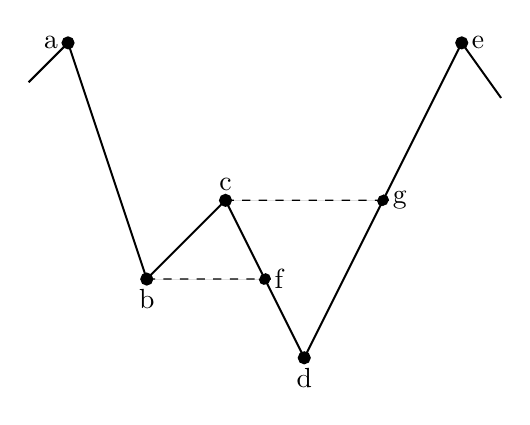
\begin{tikzpicture}
% \draw (0,0) -- (1,-3) -- (2, -2) -- (3, -4) -- (5, 0) ;
\filldraw [line width=0.25mm]
(-0.5, -0.5) --
(0,0) circle (2pt) node[left] {a} --
(1,-3) circle (2pt) node[align=center,   below] {b} -- 
(2, -2) circle (2pt) node[above] {c} -- 
(3, -4)  circle (2pt) node[below] {d} -- 
(5, 0) circle (2pt) node[right] {e} --
(5.5, -0.7);

\filldraw [line width=0.15mm, dashed]
(2, -2) -- 
(4, -2)  circle (2pt) node[right] {g};

\filldraw [line width=0.15mm, dashed]
(1, -3) -- 
(2.5, -3)  circle (2pt) node[right] {f};
\end{tikzpicture}
\caption{Способы разбиения на вложенный цикл и внешний}
\label{fig:nested-cycle}
\end{subfigure}
\hfill
\begin{subfigure}[b]{0.45\textwidth}
\centering
\begin{tikzpicture}
% \draw (0,0) -- (1,-3) -- (2, -2) -- (3, -4) -- (5, 0) ;
\filldraw [line width=0.25mm]
(0,0) circle (2pt) node[left] {a} --
(2,-4) circle (2pt) node[align=center,   below] {b} -- 
(4, 0) circle (2pt) node[right] {c};

\filldraw [line width=0.15mm, dashed]
(1, -2) circle (2pt) node[left] {d} -- 
(3, -2)  circle (2pt) node[right] {e};
\end{tikzpicture}
\caption{Разбиение цикла на два подцикла}
\label{fig:one-cycle}
\end{subfigure}
\caption{Примеры неоднозначности разбиения на циклы}
\end{figure}

Вообще говоря, без надлежащих оговорок, даже график с единственным циклом можно разбить на несколько циклов: на Рисунке \ref{fig:one-cycle} цикл $a-b-c$ разбивается на два цикла $a-de-c$ и $d-b-e$.
Очевидно, что подобным образом можно получить бесконечное количество разбиений одного цикла на любое число циклов.

В обоих рассмотренных выше примерах дополнительные варианты разбиения имели меньшую глубину внешнего цикла, чем некоторый экстремальный вариант.
Предполагая, что циклы меньшей глубины в меньшей степени расходуют ресурс накопителя, мы хотели бы получить разбиение, которое сохраняет максимально глубокие циклы.
Исторически алгоритмы rainflow, к одному из вариантов которого мы сейчас приближаемся, разрабатывались для анализа усталостных нагрузок металлов при циклических деформациях, при которых влияние на ресурс также зависит от глубины деформации.
Но в настоящее время использвуется и для анализа деградации аккумуляторных батарей в научной литературе \cite{xu2016modeling}.

Пожалуй, проще описать алгоритм, и ввести определение ``правильного'' разбиения на циклы на основе свойств этого алгоритма, чем давать их явное математическое описание.
Так, например, в статье \cite{rychlik1987new} приводится новый алгоритм подсчёта циклов, более явная форма описания которого удобна для теоретического анализа распределений циклов, формируемых случайным процессом внешнего воздействия.
Корректность нового алгоритма обосновывается доказательством того, что он даёт тот же результат, что и алгоритм rainflow, впервые предложенный в статье \cite{matsuishi1968fatigue} без четкого математического описания постановки задачи.
Попытка простого описания алгоритма rainflow в разных формах также предпринята в работе \cite{downing1982simple}.

Сейчас мы опишем алгоритм rainflow, принимающий на вход массив $s(i)$ измерений SoC или SoE и возвращающий массив $d(i)$ глубин циклов.
При желании учитывать в модели деградации средний модуль тока за цикл, предложенный алгоритм несложно модифицировать, добавив во входные данные массив времени регистрации измерений $t(i)$, а в выходные данные~--- массив длительностей циклов $\tau(i)$.

На русском языке ``Метод дождя'' принципиально описан в Стандарте 
``МЕТОДЫ СХЕМАТИЗАЦИИ СЛУЧАЙНЫХ ПРОЦЕССОВ НАГРУЖЕНИЯ ЭЛЕМЕНТОВ МАШИН И КОНСТРУКЦИЙ И СТАТИСТИЧЕСКОГО ПРЕДСТАВЛЕНИЯ РЕЗУЛЬТАТОВ'' 
ГОСТ 25.101-83, однако перевести данное в нём описание в код~--- не самая очевидная процедура.
Здесь же мы приведём псевдокод алгоритма, а с реализацией на Python3 можно ознакомиться в репозитории-приложении к работe \hyperlink{https://github.com/niquepolice/master-thesis-code/blob/master/cycles.ipynb}{по ссылке}.

Принцип работы алгоритма следующий. 
Сначала выполняется подготовительная процедура, удаляющая горизонтальные участки из графика $s(i)$ (это нужно для того, чтобы можно было определять, является ли точка локальным экстремумом, глядя лишь на значения $s(i)$ в двух соседних точках).

Далее инициализируются два изначально пустых стека (LIFO-структура данных) $min$ и $max$ для хранения индексов локальных экстремумов.
В процессе прохода по массиву каждая точка проверяется на локальный экстремум.
Если найден локальный максимум, производится ``схлапывание'' циклов разряда-заряда: если последний найденный максимум (лежащий на вершине стека $max$) не выше текущего, то он ``схлапывается вправо''~--- из стеков $min$ и $max$ удаляется по одной точке, фиксируется цикл глубины, равной модулю разности значений $s(i)$ в удалённых точках.
Это повторяется, пока на вершине стека $max$ не окажется максимум, лежащий выше текущего. 
После этого в стек $max$ добавляется текущий максимум.
Таким образом, в стеке $max$ всегда находится возрастающая последовательность локальных масимумов (если смотреть с вершины стека).
Симметричная ситуация происходит с локальными минимумами. 


\begin{figure}[]
\centering
\begin{subfigure}[b]{0.45\textwidth}
    \centering
    \begin{tikzpicture}
    % \draw (0,0) -- (1,-3) -- (2, -2) -- (3, -4) -- (5, 0) ;
    \filldraw [line width=0.25mm]
    (-0.5, -0.5) --
    (0,0) circle (2pt) node[left] {a} --
    (1,-3) circle (2pt) node[align=center,   below] {b} -- 
    (2, -2) circle (2pt) node[above] {c} -- 
    (3, -4)  circle (2pt) node[below] {d} -- 
    (5, 0) circle (2pt) node[right] {e} --
    (5.5, -0.7);
    
  \draw[-{Latex[length=3mm, width=2mm]}, dashed]
  (2,-2) -- (2/3, -2);
    \end{tikzpicture}
    % \caption{Способы разбиения на вложенный цикл и внешний}
\end{subfigure}
\begin{subfigure}[b]{0.45\textwidth}
    \centering
    \begin{tikzpicture}
    % \draw (0,0) -- (1,-3) -- (2, -2) -- (3, -4) -- (5, 0) ;
    \filldraw [line width=0.25mm]
    (-0.5, -0.5) --
    (0,0) circle (2pt) node[left] {a} --
    (1.5, -2) circle (2pt) node[above] {c} -- 
    (2.25,-3) circle (2pt) node[align=center,   below] {b} -- 
    (3, -4)  circle (2pt) node[below] {d} -- 
    (5, 0) circle (2pt) node[right] {e} --
    (5.5, -0.7);
    
  \draw[-{Latex[length=3mm, width=2mm]}, dashed]
  (5,0) -- (0, 0);
    \end{tikzpicture}
    % \caption{Способы разбиения на вложенный цикл и внешний}
\end{subfigure}

\caption{``Схлапывание'' в алгоритме rainflow.}
\label{fig:cycles-сollapse}
\end{figure}

Для примера рассмотрим ситуацию на Рисунке~\ref{fig:cycles-сollapse}.
При достижении минимума в точке b и максимума в точке $c$ ``схлапываний'' не происходит,
%~--- предыдущий максимум в точке $a$ выше текущего, в 
локальные экстремумы просто помещаются в  соответствующие стеки.
При достижении минимума в точке $d$, лежащего ниже точки $b$, 
индексы,  соответствующие точкам $b$ и $c$ удаляются из стеков,
вложенный цикл $c'-b-c$ как бы ``схлапывается влево'', 
оставляя один внешний цикл $a-d-e$, который затем ``схлопнется'' при достижении точки $e$. 

Если повернуть Рисунок \ref{fig:cycles-сollapse} на $\pi/2$, то картина схлапывающихся циклов может напомнить стекание воды по крышам пагоды (Рисунок \ref{fig:pagoda}).
Алгоритм rainflow, описанный через стекание воды по крышам пагоды, называется \textit{Pagoda roof method}.
Именно таким образом алгоритм вводится в ГОСТ 25.101-83.

\begin{figure}
    \centering
    \includegraphics[scale=0.3]{pics/pagoda.png}
    \caption{Фотография пагоды. Изображение взято с сайта https://www.pinterest.cl/pin/405394403957944422/}
    \label{fig:pagoda}
\end{figure}

\begin{algorithm}
\caption{Алгоритм Rainflow}\label{alg:rainflow}
\hspace*{\algorithmicindent} \textbf{Input:} s(i)~--- анализируемый массив, n~--- количество элементов в массиве \\
\hspace*{\algorithmicindent} \textbf{Output:} d(i)~--- массив глубин циклов 
\begin{algorithmic}[1]
% \State $cycles, i, l, h \gets 0$

\State $i,k \gets 1$
\While{$i < n$} \Comment{удаляем горизонтальные участки}
\If {$s(i) \neq s(i-1)$}
    \State $s(k) \gets s(i)$ 
    \State $k \gets k + 1$
\EndIf
\State $i \gets i + 1$
\EndWhile
\State{$n = k$}
\Statex

\Function{collapse\_last}{$max, min, s$} \Comment{``Схлапывает'' последний цикл, возвращает его глубину}
\State{$depth \gets s(max$.pop())$ - s(min$.pop())}
\State{\textbf{return} $depth$ }
\EndFunction
\Statex

\State{$i \gets 1$}
\State{$d \gets$ пустой список/массив}
\State{$min, max \gets$ пустые стеки}
\While{$i < n-1$}
\If{$s(i) > s(i-1) \And s(i) > s(i+1)$}
    \While{$max$ не пуст $\And s(i) >= s(max$.top()) } \Comment{Сравниваем текущее значение со значением предыдущего максимума}
        \State{$d$.append(COLLAPSE\_LAST($max, min, s$))} 
    \EndWhile
    \State{$max$.append($i$)}
\EndIf
\If{$s(i) < s(i-1) \And s(i) < s(i+1)$}
    \While{$min$ не пуст $\And s(i) <= s(min$.top()) } 
        \State{$d$.append(COLLAPSE\_LAST($max, min, s$))}
    \EndWhile
    \State{$min$.append($i$)}
    
\EndIf
\State{$i \gets i + 1$}
\EndWhile
 
\end{algorithmic}
\end{algorithm}

\end{enumerate}

Теперь приведём сравнение результатов применения обоих методов подсчёта циклов.

Для анализа использовался массив SoE опорной батареи (см Рисунок \ref{fig:core-cycles-line}), полученный путем моделирования на RTDS работы энергосистемы, состоящей из ветрогенератора, постоянной нагрузки, опорной батареи и нескольких других накопителей (модель разрабатывалась в рамках проектов Инжинирингового центра автономной энергетики МФТИ).
Моделирование длилось около 6 часов, для анализа использовались записи измерений с периодом 1 секунда.

\begin{figure}[h]
\includegraphics[scale=0.55]{/cycles_soe.png}
\caption{График SoE опорной батареи, использовавшийся в качестве входных данных для тестирования алгоритмов подсчёта циклов}
\centering
\label{fig:core-cycles-line}
\end{figure}

\medskip

Гистограмма глубин циклов, полученная алгоритмом Rainflow, представлена на Риснуке \ref{fig:cycles-hyst}.
По ней можно получить представление о характере работы опорной батареи в системе.
Видно, что распределение циклов практически однородное от циклов нулевой глубины до циклов максимальной глубины в ~1.5\% за исключением пика распределения около нуля, который может быть связан с шумом в измерениях.

\begin{figure}[h]
\includegraphics[scale=0.7]{/cycles_hyst.png}
\caption{Гистограмма глубин циклов, полученная алгоритмом Rainflow}
\centering
\label{fig:cycles-hyst}
\end{figure}


\begin{figure}[h]
\includegraphics[scale=0.55]{/cycles_two_methods.png}
\caption{Результаты подсчёта количества циклов глубины более $d$ двумя методами}
\centering
\label{fig:cycles-two-methods}
\end{figure}


\begin{figure}[h]
\includegraphics[scale=0.55]{/cycles_two_methods_2.png}
\caption{Результаты подсчёта количества циклов глубины более $d$ методом точечной оценки с разбиением по экстремумам и алгоритмом Rainflow с подсчетом остаточных циклов}
\centering
\label{fig:cycles-two-methods-2}
\end{figure}

Результаты подсчёта количества циклов глубины более $d$ (величины $n(1 - F(d))$) представлены на Рисунке \ref{fig:cycles-two-methods}.
Видно, что для циклов большой глубины результаты упрощённого метода, хотя и менее детализированы, но примерно совпадают c результатами Rainflow.
Но количество подсчитанных циклов малой глубины различается практически в два раза.
Это связано с тем, что простой Алгоритм \ref{alg:simple-cycle} разбивает циклы на два цикла меньшей глубины.
Например, если $s(t)$~--- треугольная повторяющаяся волна, Алгоритм \ref{alg:simple-cycle} для $d=0$ подсчитает по одному циклу вокруг каждого экстремума (получатся чередующиеся циклы заряда-разряда и разряда-заряда в два раза меньшей глубины, чем амплитуда колебаний), и подсчитанное количество циклов будет в два раза больше числа длин волн в $s(t)$.
Чтобы исправить этот недостаток, можно проверять условие завершения цикла только в локальных экстремумах.
Ниже приведён Алгоритм \ref{alg:simple-cycle-extremums}~--- модифицированный с учетом этого замечания вариант Алгоритма \ref{alg:simple-cycle}.




\begin{algorithm}
\caption{Точечная оценка $n(1 - F(d))$, разбиение по экстремумам} \label{alg:simple-cycle-extremums}
\hspace*{\algorithmicindent} \textbf{Input:} s(i)~--- анализируемый массив без подряд идущих повторяющихся значений (горизонтальных участков на графике), n~--- количество элементов в массиве, d~--- минимальная глубина цикла \\
\hspace*{\algorithmicindent} \textbf{Output:} cycles~--- количество циклов глубины более d.

\begin{algorithmic}[1]
\State $cycles, l, h \gets 0$
\State $i \gets 1$

\While{$i < n - 1$}

\If{$s(i) > s(i-1) \And s(i) > s(i+1)\Or s(i) < s(i-1) \And s(i) < s(i+1)$}
    \If {$s(h) - s(l) > d \And (l > h \And s(i) - s(l) > d \Or 
    l < h \And s(h) - s(i) > d)   $}
        \State $l,h \gets i$
        \State $cycles \gets cycles +1$
    \Else
        \If {$s(i) > s(h)$}
            \State $h \gets i$
        \EndIf
        \If {$s(i) < s(l)$}
            \State $l \gets i$
        \EndIf
    \EndIf
\EndIf
\State $i \gets i+1$
\EndWhile
 
\end{algorithmic}
\end{algorithm}

Небольшое превышение количества подсчитанных Алгоритмом \ref{alg:simple-cycle} глубоких циклов по сравнению с Алгоритмом \ref{alg:rainflow} (Rainflow) связано с тем, что после окончания работы Алгоритма \ref{alg:rainflow} в стеках $min$ и $max$ остаются вершины, ещё не ``схлопнутые'' в какой-либо цикл. 
Обычно этот ``остаток'' не накапливается при увеличении длины массива $s(i)$, поэтому для достаточно больших массивов им можно пренебречь, что и сделано в Алгоритме \ref{alg:rainflow}, чтобы не заниматься интерпретациями этих ``остатков''.
Однако для более справедливого сравнения двух методов, добавим в конец  Алгоритма \ref{alg:rainflow} подсчет оставшихся неучтенными циклов:
\begin{algorithmic}
\While{$min$ не пуст $\And max$ не пуст} 
\State{$d$.append(COLLAPSE\_LAST($max, min, s$))}
\EndWhile
\end{algorithmic}

Результаты сравнения Алгоритма \ref{alg:simple-cycle-extremums} и алгоритма Rainflow с подсчетом остаточных циклов представлены на Рисунке \ref{fig:cycles-two-methods-2}.
Теперь полученные обоими методами кумулятивные распределения глубин циклов практически совпадают.
Заметно, что расчеты Rainflow значительно детализированнее, кроме того он вычислительно эффективнее: однопоточная имплементация на Python3 требует для вычисления методом Rainflow в среднем около 0.15 секунд Intel® Core™ i7-8700, а расчёт 20 точек методом точеченой оценки~---1.7 cекунды.
